\subsection{PID - Recap}
\subsection{PID - Tuning}
    \subsubsection{\r{A}ström-Hägglund Verfahren}
        Man spezifiziert seinen Regler anhand $k_p^*, T^*, |P(0)|$. Zusätzlich kann man zwischen einem aggressiven Regler ($\mu_{min} \approx 0.5$) oder einem robusten Regler ($\mu_{min} \approx 0.7$) auswählen.
        
        \[\{k_p^*,\ T^*,\ |P(0)|,\ \mu_{min}\} \rightarrow \{k_p,\ T_i,\ T_d\}\]
            \begin{center}
            \begin{tabular}{c|c c c|c c c}
                & & $\mu_{min} = 0.7$ & & &  $\mu_{min} = 0.5$ & \\ 
                x & $\alpha_{0,x}$ & $\alpha_{1,x}$ & $\alpha_{2,x}$ & $\alpha_{0,x}$ & $\alpha_{1,x}$ & $\alpha_{2,x}$ \\ \hline
                $k_p/k_p^*$  & 0.053 & 2.90 & -2.60 & 0.13 & 1.90 & -1.30 \\
                $Ti/T^*$ & 0.90 & -4.40 & 2.70 & 0.90 & -4.40 & 2.70\\ 
                $a$  &  1.10  &  -0.0061  &  1.8  &   0.48  &  0.40  &  -0.17\\
            \end{tabular}
            \r{A}ström-Hägglund Koeffizienten für PI-Regler

        
            \begin{tabular}{c|c c c|c c c}
                & & $\mu_{min} = 0.7$ & & &  $\mu_{min} = 0.5$ & \\ 
                x &
                $\alpha_{0,x}$ & $\alpha_{1,x}$ & $\alpha_{2,x}$ & $\alpha_{0,x}$ & $\alpha_{1,x}$ & $\alpha_{2,x}$ \\ \hline
                $k_p/k_p^*$  & 0.33 & -0.31 & -1.00 & 0.72 & -1.60 & 1.20 \\
                $Ti/T^*$ & 0.76 & -1.60 & -0.36 & 0.59 & -1.30 & 0.38 \\
                $T_d/T^*$ & 0.17 & -0.46 & -2.10 & 0.15 & -1.40 & 0.56\\
                $a$  &  0.58  &  -1.3000  &  3.5  &   0.25  &  0.56  &  -1.20\\
            \end{tabular}    
            \r{A}ström-Hägglund Koeffizienten für PID-Regler 
            
            \end{center}
            
            mit diesen Parametern können wir $\square \in \{a, k_p,\, T_i,\, T_d\}$ bestimmen.
            \[ \square = \square^* \cdot \alpha_{0,x} \cdot e^{\alpha_{1,x} \cdot \kappa + \alpha_{2,x} \cdot \kappa^2}
            \ \textnormal{mit} \ \kappa = \frac{1}{|P(0)| \cdot k_p^*} \]
            \textbf{Note:}
            \begin{itemize}
                \item $T^* = T_i^*,\  T_d^*$ oftmals gibt \r{A}ström-Hägglund Verfahren bessere Resultate als Ziegler-Nichols. Dies ist jedoch nicht immer der Fall. 
                \item Beim set point weight $a$ wählt man für $a^* = 1$ 
            \end{itemize}
            
    \subsubsection{Direktspezifikationen} 
        Ziel der Direktspezifikation ist die PID- parameter so zu wählen, dass die Kreisverstärkung die gewünschte \textbf{Übergangsfrequenz $\omega_c$}, \textbf{Phasenereserve} $\varphi$ und \textbf{Steigung} $\psi$ erzielt. Zusätzlich brauchen wir noch 
        \begin{align*}
        r_P &= |P(j\omega_c)|   &   \varphi_P &= \angle P(j\omega_c)\\
        r'_P &= \frac{\partial r_P(\omega)}{\partial\omega}\Bigg|_{\omega=\omega_c} & \varphi'_P &= \frac{\partial \varphi_P(\omega)}{\partial\omega}\Bigg |_{\omega=\omega_c}
        \end{align*}
        Mit diesen Werten können wir nun die PID-Parameter bestimmen:
        \[k_P = - \frac{1}{r_P}\cos(\varphi-\varphi_P)\]
        \begin{multline*}
        T_d =\frac{1}{2}\cdot\Bigg(\tan(\psi-\varphi_P)\Bigg(\frac{r'_P}{r_P}-\varphi'_P\tan(\varphi-\varphi_P)\Bigg)\\ + \tan(\varphi-\varphi_P) \Bigg(\frac{1}{\omega_c}-\frac{r'_P}{r_P}\Bigg)- \varphi'_P\Bigg)
        \end{multline*}
        \[T_i = (T_d\cdot \omega_c^2 - \tan(\varphi-\varphi_P)\cdot \omega_c)^{-1}\]
        \textbf{Note:} Die Stabilität ist mit diesem Verfahren nicht garantiert. Phase muss in der Formel in Radiant angegeben werden. 
\subsection{Prädikative PI Regler}
    für Regelstrecken mit wesentlicher Totzeit, das heisst falls 
    \[\frac{T}{T+\tau}>0.3\]
    kann man nicht einfach einen PID-Regler auslegen. Stattdessen legt man einen Controller aus der mit der Totzeit umgehen kann. 

    
    \subsubsection{Prädikative PI Regler für einfache Regelstrecken}
        Annahme: Regelstrecke erster Ordnung 
        \[P(s)\approx \frac{k}{\tau s + 1}\cdot e^{-Ts}\]
        man wählt die gewünschte \textbf{Sensitivität} 
        \[S(s) = 1- \frac{1}{s\cdot\sigma\cdot \tau + 1 \cdot e^{-Ts}} = 1 - T(s) \]
        mit $\sigma = $ Tuning-Parameter
        Der Kontroller der die gewünschte Kreisverstärkung erfüllt hat folgende Form 
        \[C(s) =\frac{1-S(s)}{S(s)\cdot P(s)}= \frac{\tau\cdot s+1}{k\cdot(\sigma\cdot\tau\cdot s+ 1-e^{-Ts})}\]
        Somit lautet die Eingangsgrösse: 
        \[U(s)=\underbrace{\frac{1}{\sigma k}\Bigg(1+\frac{1}{\tau\cdot s}\Bigg)E(s)}_{\textnormal{PI-Regler}} - \underbrace{\frac{1}{\sigma\tau s}(1-e^-{Ts})\cdot U(s)}_{\textnormal{Prädikitve Korrektur}}\] 
    \textbf{Note:} Falls T = 0 wird die prädikative Korrektur 0 und der resultierende Eingang wird zu einem einfachen PI - Regler.
    \subsubsection{Smith Predictor}
    Annahme: System hat einen rationalen Teil und eine Totzeit
    
    \[P(s) = P_r(S)\cdot e^{-Ts}\]
    \begin{figure}[H]
        \centering
        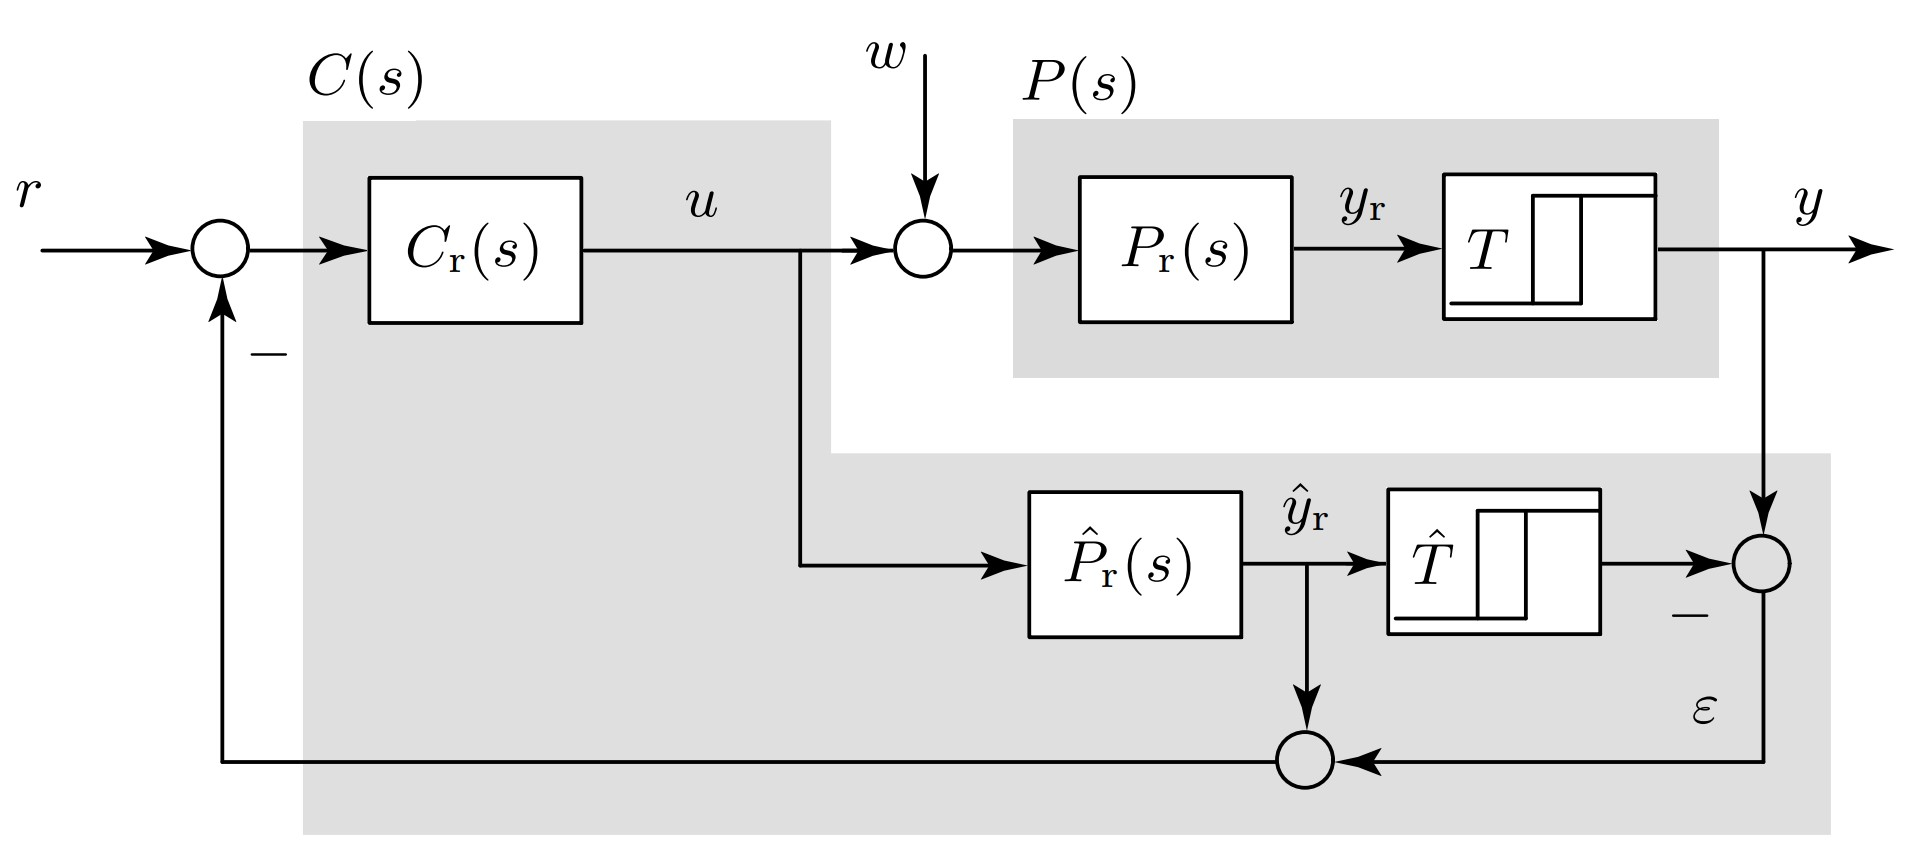
\includegraphics[width = 0.7\linewidth]{images/02/Smithpredictor.jpg}
        \caption{Regelstruktur eines Smith Predictors}
    \end{figure}
    
    wenn es keine Modellfehler gibt ($P_r(s) = \hat P_r(s),\ T = \hat T$) und keine Störung ($\omega = 0$)($\Rightarrow \epsilon = 0$), resultiert folgende komplementäre Sensitivität:
    \begin{align*}
        L_{\textnormal{pred}} &= \frac{C_r(s)}{1 + C_r(s)\cdot\hat{P}_r(s)\cdot\big(1 - e^{-s\hat{T}}\big)}\cdot P_r(s)\cdot e^{-sT}\\
        \frac{Y(s)}{R(s)} &= e^{-Ts}\cdot\frac{P_r(s)C_r(S)}{1+P_r(S)C_r(s)} = e^{-Ts}\cdot T_r(S)
    \end{align*}
    Auflösen der obigen Gleichung nach $C(s)$ liefert
    \begin{equation*}
        C_r(s) = \frac{T_{\textnormal{ref}}(s)}{P_r(s)\cdot(1-T_{\textnormal{ref}}(s))}
    \end{equation*}
    wobei $T_\textnormal{ref}(s)$ die gewünschte TF von $r\rightarrow y$ ist.
    
    \textbf{Note:} 
    \begin{itemize}
        \item Falls Modellfehler und Störungen vorhanden sind wird die Gleichung für die komplementäre Sensitivität wesentlich komplizierter!
        
        \item Nicht miniphasige NST von $P(s)$ werden zu instabilen Polen 
    \end{itemize}
    
    Schätzungsfehler von der Totzeit $T$ kann grosse Auswirkungen auf das Systemverhalten haben. Bei einem Schätzfehler von $\pm 20\%$ kann immer noch eine schnelle und robuste Systemantwort ohne übermässige Abweichungen vom Referenzsystem erzielt werden.
    \begin{figure}[H]
        \centering
        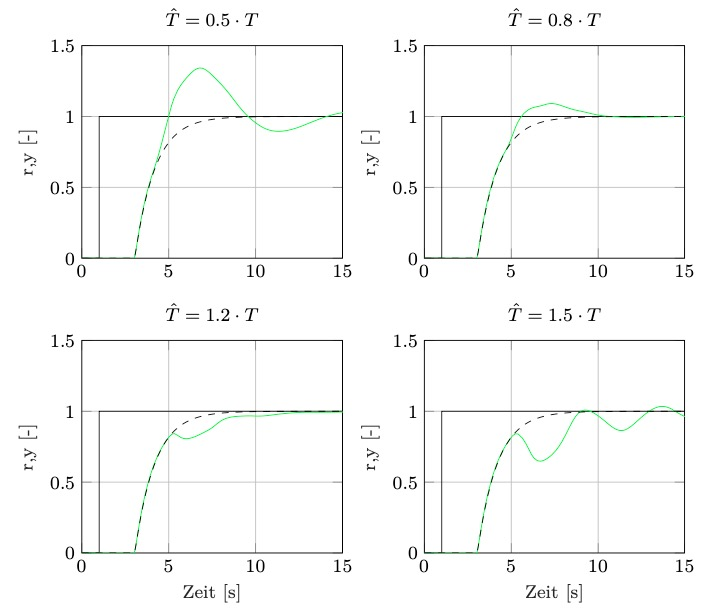
\includegraphics[width = 0.9\linewidth]{images/02/est_error_hat_T.jpg}
        \caption{Auswirkung Schätzungsfehler von $\hat{T}$ auf die Sprungantwort}
    \end{figure}
    
